\lhead{\begin{tikzpicture}[remember picture, overlay]
    \node [anchor=100,inner sep=0] (imagenIZQUIERDA) at (current page header area.north){
\includegraphics[width=18cm]{19/Img/encabezado.PNG}};
    \end{tikzpicture}}
    \rhead{Nieto-Leal}
    \rfoot{\begin{tikzpicture}[remember picture, overlay]
    \node [anchor=140,inner sep=0] (imagenDERECHA) at (current page footer area.south){
\includegraphics[width=18cm]{19/Img/foot.PNG}};
    \end{tikzpicture}}
    %----------------------------------------------------------------------------------------
    \lfoot{ \thepage}
    % \renewcommand{\labelenumi}{\alph{enumi}.)} 
    %----------------------------------------------------------------------------------------
    %----------------------------------------------------------------------------------------
    %	TITLE SECTION
    %----------------------------------------------------------------------------------------
    
    \setlength{\droptitle}{-5\baselineskip} % Move the title up
    \title{\textbf{Estudio de tiempos y movimientos en el ensamble de un circuito electrónico utilizando diferentes métodos para su optimización }} % Article title
    
     \author{ 
     \textsc{Nieto-Leal, Emiliano }\\ 
    %  Afiliación:
     \texttt{ Instituto Tecnológico de Querétaro } \\ 
     \texttt{Tecnológico Nacional de México } \\ 
     \texttt{Querétaro, México}\\ 
     \texttt{l22140880@queretaro.tecnm.mx} 
     \and 
     \textsc{Ángeles-Hurtado, Luis Alberto}\\ 
    %  Afiliación:
     \texttt{ Instituto Tecnológico de Querétaro } \\ 
     \texttt{ Tecnológico Nacional de México } \\ 
     \texttt{Querétaro, México}\\ 
     \texttt{alb3rt0.ah@gmail.com} 
    }
    
    
    %----------------------------------------------------------------------------------------
    
    % \begin{document}
    
    % Print the title
    \maketitle
    \thispagestyle{fancy}
    
    %----------------------------------------------------------------------------------------
    %	ARTICLE CONTENTS
    %----------------------------------------------------------------------------------------
    
    % \section*{Resumen}
    % \textit{Palabras clave:}
    % El resumen (ancho de página) deberá contener entre 100 y 200 palabras tipo Adobe Devangari 11 puntos.
    
    \begin{abstract}
    \noindent 
    El resumen (ancho de página) deberá contener entre 100 y 200 palabras tipo Adobe Devangari 11 puntos.
    
    \end{abstract}
    % 
    % 
    \textbf{\textit{Palabras clave}}: {Tiempo, Movimiento, Medición, Muestreo, Registro y Opti.}
    % \keywords{First keyword should be the corresponding to the research area according with the authors guide. Maximum of 6 keywords.}
    
    \section{Introducción}
    
    
    \begin{itemize}
        \item En la industria siempre se necesita de una mejora continua, por lo que a la hora de empezar trabajos como en ensamblaje (los cuales requieren de varias piezas y herramientas a utilizar) o para poder acelerar los tiempos de producción y minimizar los movimientos para el trabajo, es necesario que cualquier analista entienda las bases de los métodos diseñados para su estudio, siendo el principal de estos el estudio de tiempos y movimientos.\cite{RAE}
        \\En líneas generales el estudio de tiempos y movimientos es una herramienta que permite el analizar todo aquello que de alguno u otra manera tenga relación o afecte al trabajo que se plantea en el estudio(siendo estos los métodos, materiales, herramientas a usar y las instalaciones donde se trabajara), permitiendo separar todos estos factores para su estudio detallado y así buscar optimizar el trabajo estudiado.
        \\Siendo la optimización no solo el objetivo mas importante de estos métodos sino un concepto que siempre se debe de considerar y procurar en todo momento. Al ser " la selección de una alternativa mejor, en algún sentido, que las demás alternativas posibles"\cite{Pontificia2001}, por lo que en síntesis cualquier analista buscara la opción de entre todas las posibles que le genere alguna especie de beneficio en un rasgo en especifico del proyectos. Sumado al estudio de tiempos y movimientos hay mas metodologías que permiten la optimización de las operaciones, estando tanto los estudios de tiempo, en el cual  se busca obtener el valor esperado de cuanto tiempo tomará realizar una actividad, el muestreo de trabajo el cual con base en una muestra elegida de operadores podemos obtener los porcentajes de tiempos productivos, y principalmente los sistemas de tiempo predeterminados, los cuales tienen como propósito dividir los trabajos en elementos y que con ayuda de unas tablas podemos calcular y asignar un tiempo para cada uno de estos elementos, de esta manera llegando a obtener el tiempo total de la operación.\cite{EstTrabajo}
        \\Por ello para entender de mejor manera como es que se utilizan diversas metodologías y herramientas relacionadas a optimización de los procesos de fabricación se deberá determinar el tiempo productivo y no productivo que un operario (en este caso un compañero) realizara en relación al ensamblaje de un circuito eléctrico. Con ensamble nos referimos a la unión de varias piezas eléctricas, usando un "Protoboard como base para circuito eléctrico, el cual es un conjunto de componentes eléctricos utilizados en la generación y transmisión de energía eléctrica para un propósito en especifico.\cite{CircElec}
        Por lo que usando diversos metodologías para poder obtener los valores del tiempo productivo de nuestros compañeros, creando un registro histórico de estos valores y así poder realizar una comparación entre los métodos utilizados, para de esta manera no solo obtener mayor experiencia en su uso, también observando cual método se adecua mas para cada situación.
    
    \end{itemize}
    % 
    % 
    \section{Justificación}
    
    \begin{itemize}
        \item A día de hoy debido a los grandes avances en tecnología y a la cercanía del mundo entero debido a herramientas como el internet y las redes sociales han generado una globalización que ha afectado a cualquier tipo de mercado existente, por ello mismo la gran competencia entre productos también ha ido en aumento, viendo como todas las empresas quieren encontrar la manera de destacar por sobre sus competidores, algunas de ellas a través de la publicidad y otras por medio de la calidad de sus productos, siendo en este aspecto donde entra el analista. Para lograr que estos productos lleguen a más gente y sean considerados mas que sus competencias es importante tener un buen analista, ya que al desarrollar un pensamiento racional y analítico, sumado a sus habilidades de comunicación y al uso de metodologías de optimización estos deberán de garantizar la calidad del producto, y por ende la satisfacción del cliente. Buscando utilizar la forma mas óptima de realizar todos los procesos y a su vez sin que estos incumplan cualquier tipo de estandarización o que afecte a la calidad del producto.\cite{Indeed}
    \end{itemize}
    % 
    % 
    \section{Descripción del problema}
    \begin{itemize}
        \item El análisis de tiempos y movimientos como presente anteriormente es una de las herramientas mas utiles y esencials que cualquier operario debe tener para poder realizar de manera adecuada su trabajo, pero no solo debe de quedarse ahi, ya que debido a la alta tasa de competititvidad es impiortante mantenerse a la vanguardia de de todo nueva metodologia o herramienta que pueda no solo facilitar su trabajo sino tambien y principalmente generar un beneficio hacia la compañia.
        \\
    
        \item Se debe describir la desviación o diferencia del ``es'' con respecto al ``debe ser''.
        \item Se debe hacer alusión a la incógnita científica*.
        \item Debe de tener Referencias científicas, URL, tesis, etc.
    \end{itemize}
    
    \textbf{*La incógnita científica es el elemento cuya solución incrementa el conocimiento científico.}
    % 
    % 
    \section{Fundamentación teórica}
    
    Es la parte medular y de mayor discusión, deberá ser la fundamentación de la hipótesis, por tanto se deberá señalar claramente la razón de la suposición y fundamentación de la misma. Únicamente referencias científicas.
    \begin{itemize}
        \item Se debe de retomar el tema que se planteo en la introducción, pero ahora profundizando para clarificar la incógnita científica y se pueda plantear la hipótesis.
        \item Se debe de retomar la descripción del problema, pero ahora a profundidad del (los) objeto(s) de estudio. 
        \item Se debe de profundizar en las metodologías que se ha usado para el estudio del tema.
        \item Referencias solo de artículos y libros científicos.
    \end{itemize}
    % 
    % 
    \section{Hipótesis}
    
    Es la suposición con fundamento científico relativa a la solución del problema, necesidad o de cómo se aprovecha la oportunidad con la incógnita científica y se fundamenta con: 1. Una suposición (en afirmativo o negativo) y ésta deberá vincularse con:
    2. La fundamentación científica que deberá ser precisa 3. Una entidad de comparación para probar la suposición y
    4. La variable con que se califica o cuantifica la comparación o se prueba la hipótesis.
    
    \begin{itemize}
        \item Se debe de identificar claramente la suposición científica
        \item Se debe de identificar claramente el fundamento científico
        \item Se debe identificar claramente la variable de respuesta
        \item Se debe identifican claramente las realidades o modelos contrastantes
        \item Se debe de establecer las variables asociadas, explicativas o que tienen relación funcional con la variable de respuesta
    \end{itemize}
    % 
    % 
    \section{Objetivo}
    
    Precisar la acción necesaria para probar la hipótesis. Dicha acción se establece mediante el uso de verbos activos y en infinitivo.
    \begin{itemize}
        \item Se debe establecer que se pretende probar la hipótesis
    \end{itemize}
    
    \subsection{Objetivos específicos }
    
    \begin{itemize}
        \item Se debe establecer como un conjunto de acciones comunes para lograr el objetivo general
        \item Se debe establecer como etapas para lograr el objetivo general
    \end{itemize}
    
    Son actividades orientadas al cumplimiento del objetivo general. Se establecen con verbos activos en infinitivo. Son parte de la acción encaminada a probar la hipótesis. Éstos deben ser precisos, y en lo posible evitar aspectos metodológicos.
    % 
    % 
    \section{Cuerpo (Metodología, modelo matemático, etc.)}
    
    Cada estrategia metodológica se establece acorde a cada objetivo, y por tanto deberá ser desglosada precisada y ordenada claramente. En consecuencia cada objetivo que se presentó en forma de verbo en infinitivo deberá determinar una estrategia en forma de adverbio. Ej. Desarrollar…Desarrollo. Son las actividades ordenadas que tienen como finalidad la prueba de la hipótesis. 
    
    \begin{itemize}
        \item Se debe establecer que se habrá de hacer, como, conque, y donde para obtener la información que permita probar la hipótesis.  
        \item Se debe desglosar de acuerdo a los objetivos específicos. 
        \item Se debe establecer una estrategia metodológica por cada objetivo específico. De manera simplista se podría decir que se cambia el verbo en infinitivo por su respectivo adverbio.
        \item En cada objetivo se debe describir que método, que materiales y que equipo se usará para conseguirlo.
        \item Se deben tener referencias Figura \ref{fig:lcd-16x2}.
    \end{itemize}
    % 
    % 
    \begin{figure}[H]
        \centering
        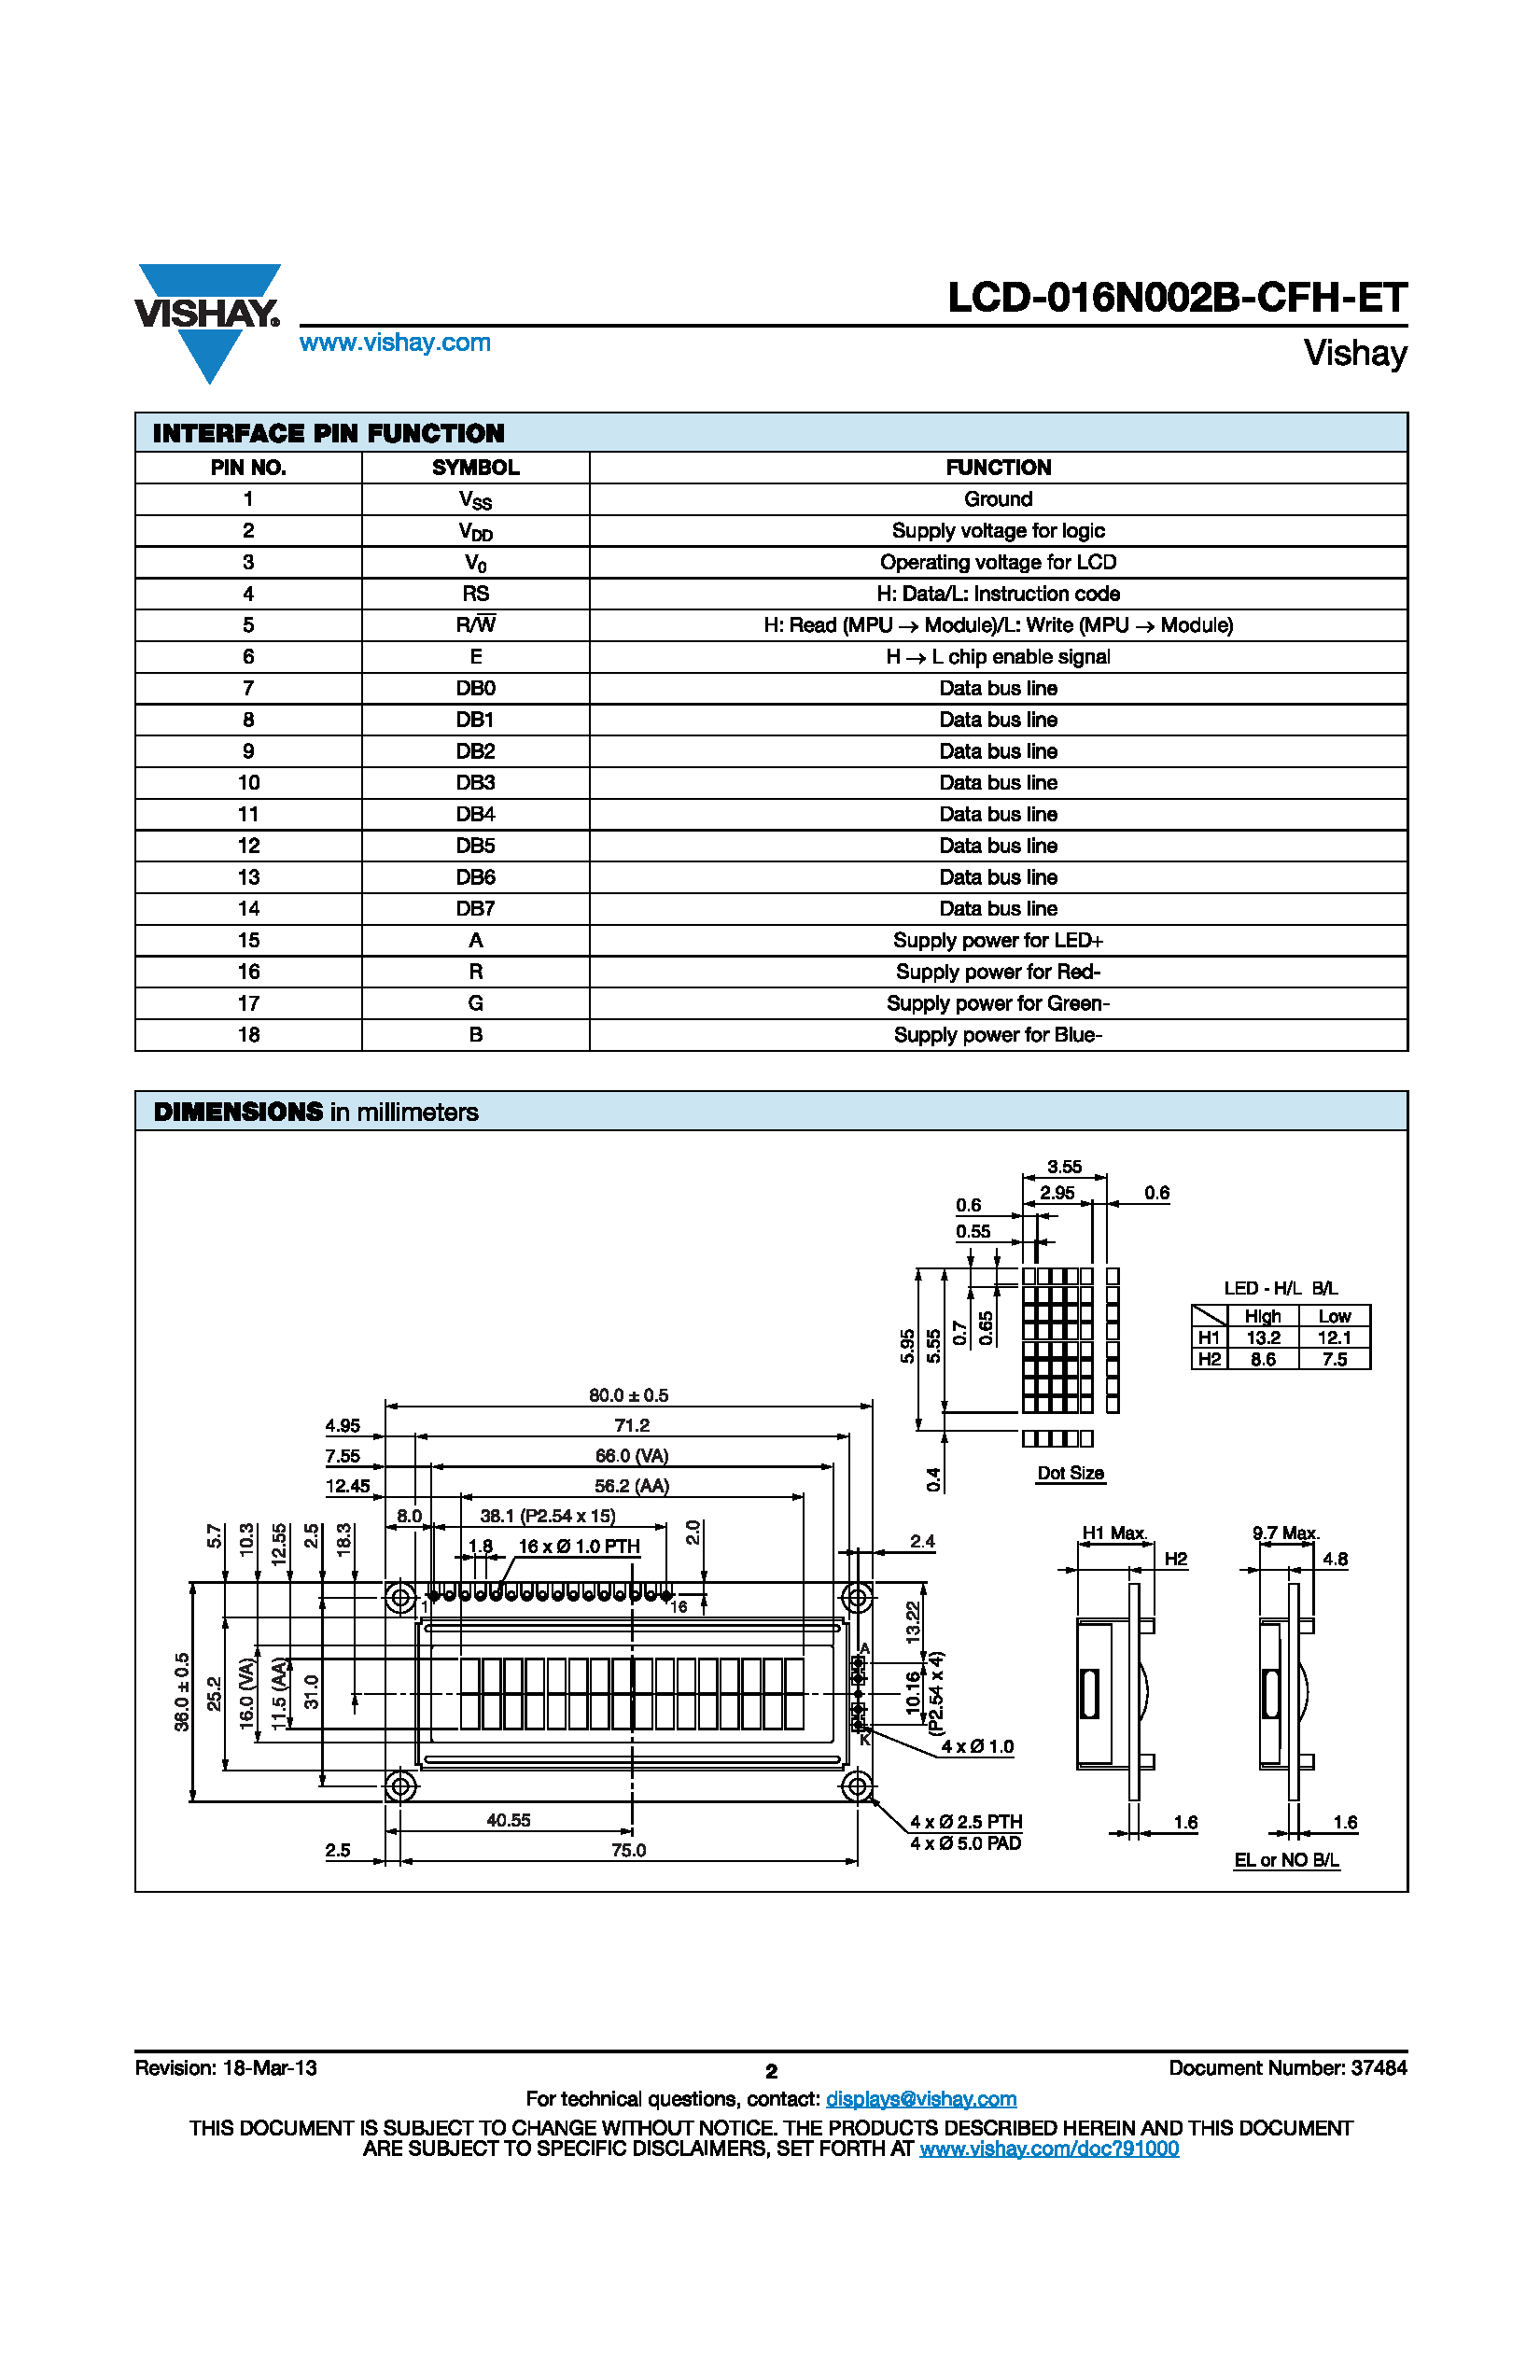
\includegraphics[trim = {30mm 65mm 90mm 250mm},clip,scale=0.5]{19/Img/lcd-16x2.pdf}
        \caption{Esquema LCD de 16x2}
        \label{fig:lcd-16x2}
    \end{figure}
    % 
    % 
    \begin{figure}[H]
        \centering
        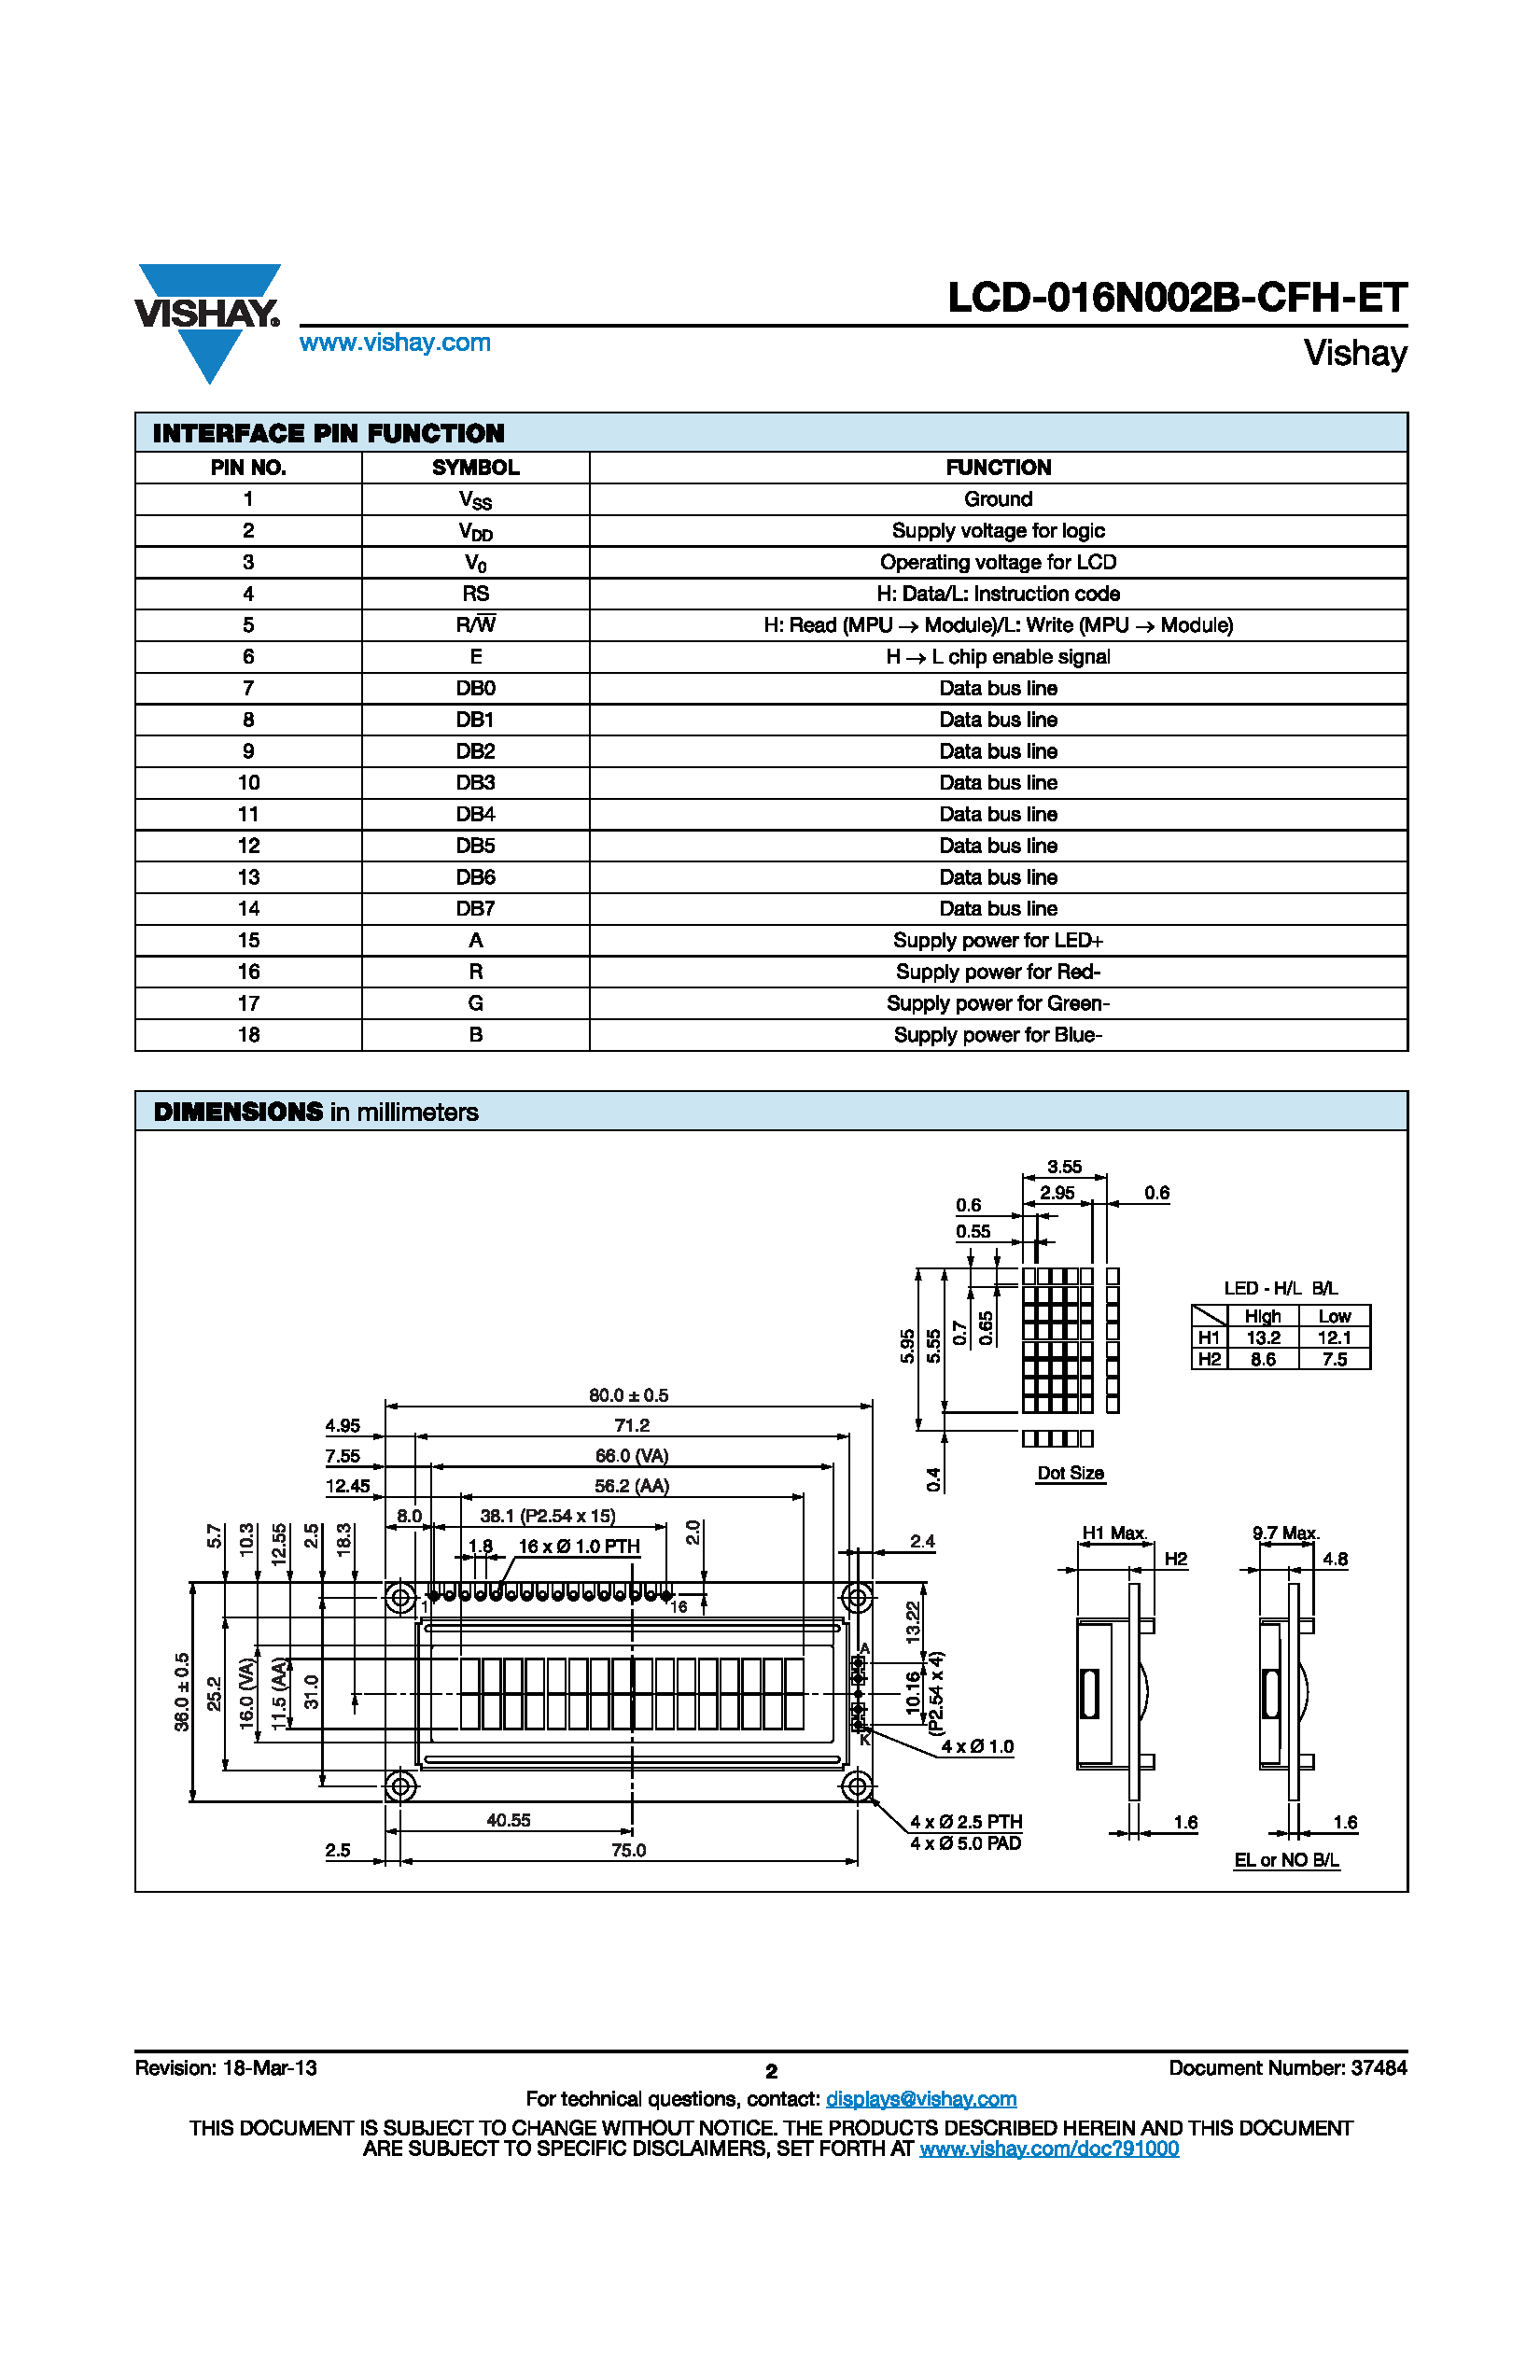
\includegraphics[trim = {30mm 250mm 90mm 20mm},clip,scale=0.5]{19/Img/lcd-16x2.pdf}
        \caption{Esquema LCD de 16x2}
        \label{fig:lcd-16x2}
    \end{figure}
    % 
    % 
    \subsection{Prepara tu documento}
    
    Antes de que comiences a utilizar esta plantilla, es recomendable que prepare la información que contendrá en un archivo aparte. 
    Ten preparadas tus gráficas, así como también las tablas aparte, para que sea más fácil integrarlo. 
    Se recomienda fuertemente el uso de \textbf{formato Enhanced Metafile (.emf) para imágenes y gráficas} de resolución óptima. 
    Finalmente, completa y organiza el contenido antes de darle el formato de esta plantilla. 
    
    \subsection{Acrónimos y Abreviaciones}
    
    Los acrónimos y abreviaciones deberán ser definidos únicamente la primera vez que aparecen en el texto, esto para que el lector entienda lo que significan.
    
    \subsection{Ecuaciones}
    
    Las ecuaciones son una excepción a las especificaciones prescritas de esta plantilla. 
    Deberá determinar si su ecuación debe escribirse o no utilizando la fuente Adobe Devangari. 
    Para crear ecuaciones multinivel, puede ser necesario tratar la ecuación como un gráfico e insertarla en el texto después de aplicar el estilo de la platilla.
    Las ecuaciones serán enumeradas de manera consecutiva, y el número de ecuación, entre paréntesis, se colocan al ras de la derecha, utilizando una tabulación derecha. 
    
    \begin{equation}
        \label{eq1}
        x + y = z 
    \end{equation}
    
    Es importante asegurarse de que los símbolos de la ecuación sean definidos antes o inmediatamente después de la ecuación. Utilice “(1)”, en vez de “Eq. 1” al enumerar las ecuaciones, excepto al principio de una oración: “La ecuación (\ref{eq1}) es…”
    
    \section{Resultados y discusión}
    
    Antes de comenzar a preparar tu artículo, es importante que lea primero la guía del autor, la cual incluye los temas o apartados que son necesarios para tener tu trabajo completo.
    Una vez completada la edición del texto, el documento está listo para el uso de esta plantilla. En este archivo recién creado, resalte todo el contenido e importe el archivo de texto preparado. Ahora esta listo para estilizar su documento.
    En esta sección se deben presentar todo lo obtenido de la sección 2, incluidas deducciones o efectos del desarrollo. También se podrán incluir subsecciones numeradas de la siguiente forma:
    
    \subsection{Autores y Afiliaciones}
    
    Para distinguir las afiliaciones de los autores, utilice superíndices iniciando con el número 1, 2, etc., sucesivamente, esto dependerá de la cantidad de los departamentos a los que estén afiliados los autores. En caso de que todos los autores pertenezcan a una mismo departamento e institución, utilizar sólo el superíndice 1. 
    
    \subsection{Identificar los encabezados}
    
    Se les recuerda a los autores que los encabezados deben de estar conforme los solicita la guía del autor. De ahí se puede adaptar el trabajo para que sea más fácil de entender para el lector.
    Los encabezados organizan los temas sobre una base relacional y jerárquica. Por ejemplo, el título del documento es encabezado del texto principal porque todo el material posterior se relaciona y elabora sobre este tema. 
    
    \subsection{Tablas y Figuras}
    
    \begin{enumerate}
        \item Posición de las tablas y figuras: Coloque las figuras y las tablas en la parte superior e inferior de las columnas. Evite colocarlos en medio. Las figuras y las tablas grandes pueden abarcar ambas columnas. Los títulos de las figuras deben de estar debajo de las mismas; los títulos de las tablas deben aparecer encima de ellas. Insértese las figuras y los cuadros después de citarse en el texto. Utilice la abreviatura “Fig. 1”, incluso al principio de una oración. 
    \end{enumerate}
    
    \section{Conclusiones}
    
    Se describe aquí el alcance del trabajo, logros obtenidos y perspectivas para el futuro de este. Se sugiere colocar información cuantitativa obtenida.
    
    \section{Agradecimientos}
    
    Es importante darles su debido reconocimiento a los laboratorios, instituciones, organizaciones, entre otros que han sido participes para la culminación de este trabajo. También es importante mencionar, fondos, proyectos, becas, entre otros que se le han otorgado al o los autores para realizar el trabajo de investigación. Ejemplo: “Los autores agradecen al Concejo Nacional de Ciencia y Tecnología por los recursos otorgados…”
    
    \section*{Referencias}
    
    Para esta platilla, se solicita al autor enumerar las citas de manera consecutiva entre corchetes \cite{GoA2015}. 
    La puntuación de la oración que sigues sería \cite{RAE}. 
    Refiérase simplemente al número de referencia, como en \cite{Morales2012}, no utilice “Ref. [3]” o “referencia [3]” excepto al principio de una oración: “La referencia [3] fue la primera…”
    Enumere las notas al pie por separado en superíndices. Coloque la nota de pie de en la parte inferior de la columna en la que se citó. No coloque notas al pie en la lista de referencias. Utilice letras para las notas al pie de la tabla.
    A menos de que haya tres autores o más; no utilice “et al.”. Los trabajos que no hayan sido publicados, incluso si han sido presentados para su publicación, deben ser citados como “inéditos”. Los trabajos que han sido aceptados para su publicación deben de citarse como “en prensa”. Poner en mayúscula sólo la primera palabra de un título, excepto los nombres propios y los símbolos de elemento. 
    
    Otros ejemplos \cite{LAAngeles2021}, \cite{LAAngelesConni}. 
    
    % Ejemplo
    %  @Article{article,
    % 	author = "Author1 LastName1 and Author2 LastName2 and Author3 LastName3",
    % 	title = "Article Title",
    % 	volume = "30",
    % 	number = "30",
    % 	pages = "10127-10134",
    % 	year = "2013",
    % 	doi = "10.3389/fnins.2013.12345",
    % 	URL = "http://www.frontiersin.org/Journal/10.3389/fnins.2013.12345/abstract",
    % 	journal = "Frontiers in Neuroscience"
    % }
    
    % @book{book,
    %   author    = {Author Name}, 
    %   title     = {The title of the work},
    %   publisher = {The name of the publisher},
    %   address   = {The city},
    %   year      = 1993,
    % }
    
    % @incollection{chapter,
    %   author       = {Bauthor Surname}, 
    %   title        = {The title of the work},
    %   editor       = {Editor Name},
    %   booktitle    = {The title of the book},
    %   publisher    = {The name of the publisher},
    %   address      = {The city},
    %   year         = 2002,
    %   pages        = {201-213},
    % }
    
    % @InProceedings{conference,
    %   author = {Cauthor Name and Dauthor Surname and Fauthor LastName},
    %   title = {The title of the work},
    %   booktitle = {The title of the conference proceedings},
    %   year = 1996,
    %   publisher = {The name of the publisher},
    %   editor = {Editor Name1 and Editor Name2},
    %   pages = {41-50},
    % }
    
    % @book{cho,
    %   author       = {Gauthor Name1}, 
    %   title        = {The title of the work},
    %   publisher = {Country code and patent number},
    %   address      = {Patent Country},
    %   year = 2013
    % }
    
    % @book{patent,
    %   author    = {Hauthor Surname1}, 
    %   title     = {The title of the work},
    %   publisher = {Patent number},
    %   address   = {Patent country},
    %   year      = 2010,
    % }
    
    % % please use misc for datasets
    % @misc{dataset, 
    % 	author = "Author1 LastName1 and Author2 LastName2 and Author3 LastName3",
    % 	title = "Data Title",
    % 	year = "2011",
    % 	doi = "10.000/55555",
    % 	URL = "http://www.frontiersin.org/",
    % }
    
    \bibliographystyle{ieeetr}
    \bibliography{19/referencias}
    % 
    % 
    %%%%%%%%%%%%%%%%%%%%%%%%%%%%%%%%%%
    \appendix
    %%%%%%%%%%%%%%%%%%%%%%%%%%%%%%%%%%
    % 
    % 
    \centering{\section[\appendixautorefname{}]{APÉNDICE}}
    \includepdf[pages=-]{19/Img/pines.pdf}
    \label{anexo:pines}
    %%%%%%%%%%%%%%%%%%%%%%%%%%%%%%%%%%%%%%%%